% Official source: https://www.imo-official.org/assets/documents/problems/2004/2004_eng.pdf
\competitionyear{2004}

\begin{problem}{2004}{1}
Let $ABC$ be an acute triangle with $AB\ne AC$. The circle with diameter $\overline{BC}$ meets the sides $AB$ and $AC$ at $M$ and $N$, respectively. Let $O$ be the midpoint of $BC$, and let the bisectors of $\angle BAC$ and $\angle MON$ intersect at $R$. Prove that the circumcircles of triangles $BMR$ and $CNR$ have a common point on the side $BC$.
\end{problem}

\begin{problem}{2004}{2}
Determine all polynomials $f$ with real coefficients such that
\[
    f(a-b)+f(b-c)+f(c-a)=2f(a+b+c)
\]
for every $a, b, c\in\R$ satisfying $ab+bc+ca=0$.
\end{problem}

\begin{problem}{2004}{3}
A \emph{hook} is the arrangement of six unit squares shown below, or any rotation or reflection of it.

% Six unit squares in the official 2004 IMO Problem 3 hook.
\begin{center}
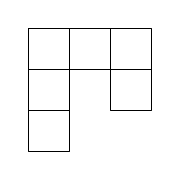
\begin{tikzpicture}[x=0.52cm,y=0.52cm,line width=0.45pt,line join=round]
    \draw (0,0)--(1,0)--(1,2)--(2,2)--(2,1)--(3,1)--(3,3)--(0,3)--cycle;
    \draw (0,1)--(1,1) (0,2)--(1,2) (2,2)--(3,2);
    \draw (1,2)--(1,3) (2,2)--(2,3);
\end{tikzpicture}
\end{center}


Determine all $m\times n$ rectangles that can be tiled with hooks, with neither gaps nor overlaps and with every hook contained in the rectangle.
\end{problem}

\begin{problem}{2004}{4}
Let $n\geq3$ be an integer and let $t_1, \dots, t_n$ be positive real numbers satisfying
\[
    (t_1+\cdots+t_n)\left(\frac1{t_1}+\cdots+\frac1{t_n}\right)<n^2+1.
\]
Prove that $t_i, t_j, t_k$ are the side lengths of a triangle whenever $1\leq i<j<k\leq n$.
\end{problem}

\begin{problem}{2004}{5}
In a convex quadrilateral $ABCD$, the diagonal $BD$ bisects neither $\angle ABC$ nor $\angle CDA$. Let $P$ be an interior point satisfying
\[
    m\angle PBC=m\angle DBA,\qquad m\angle PDC=m\angle BDA.
\]
Prove that $ABCD$ is cyclic if and only if $AP=CP$.
\end{problem}

\begin{problem}{2004}{6}
Call a positive integer \emph{alternating} if adjacent digits in its decimal expansion always have opposite parity. Determine all positive integers with an alternating multiple.
\end{problem}
